% This is the University of Chicago Graham School Master of Science in Analytics
% template. Much of it is based on the Reed College LaTeX thesis template.
% Most of the work for the Reec College template was done by Sam Noble (SN),
% Later comments etc. by Ben Salzberg (BTS).
% Additional restructuring and APA support by Jess Youngberg (JY).
% Justin M. Shea (JMS) built on their good open source work.
% Your comments and suggestions are more than welcome:
% please email, them to justinshea@uchicago.edu.
%
% Any line that starts with a percent symbol is a comment.
% They won't show up in the document, and are useful for notes
% to yourself and explaining commands.
% Commenting also removes a line from the document;
% very handy for troubleshooting problems. -BTS
%%
%% Preamble
%%
% \documentclass{<something>} must begin each LaTeX document
% Added by JMS
\documentclass[12pt,oneside]{chicagocapstone}
% END of JMS add
% Packages are extensions to the basic LaTeX functions. Whatever you
% want to typeset, there is probably a package out there for it.
% Check out CTAN to see: http://www.ctan.org/
%%
\usepackage{graphicx,latexsym}
\usepackage{amsmath}
\usepackage{amssymb,amsthm}
\usepackage{longtable,booktabs,setspace}
\usepackage[hyphens]{url}
% Added by CII
\usepackage{hyperref}
\usepackage{lmodern}
\usepackage{float}
\floatplacement{figure}{H}
% End of CII addition
\usepackage{rotating}


% Added by CII (Thanks, Hadley!)
% Use ref for internal links
\renewcommand{\hyperref}[2][???]{\autoref{#1}}
\def\chapterautorefname{Chapter}
\def\sectionautorefname{Section}
\def\subsectionautorefname{Subsection}
% End of CII addition

% Added by CII
\usepackage{caption}
\captionsetup{width=5in}
% End of CII addition

% Added by JMS
\usepackage{mathptmx} % Times New Roman fonts
% End of add by JMS

% Syntax highlighting #22

% To pass between YAML and LaTeX the dollar signs are added by CII
\title{Your Capstone Project Title}
\author{Robert Knox, Adetola Adedeji, Xiaolei Zhang}
\date{Month, Year} % The month and year that you submit your FINAL draft)
\division{Graham School}
\advisor{Arnab Bose}
\institution{University of Chicago}
\degree{Master of Science in Analytics}
\altadvisor{Dr.~Sema Barlas}
% End of CII addition

\department{Continuing Liberal and Professional Studies}

% Added by CII
%%% Copied from knitr
%% maxwidth is the original width if it's less than linewidth
%% otherwise use linewidth (to make sure the graphics do not exceed the margin)
\makeatletter
\def\maxwidth{ %
  \ifdim\Gin@nat@width>\linewidth
    \linewidth
  \else
    \Gin@nat@width
  \fi
}
\makeatother

\renewcommand{\contentsname}{Table of Contents}
% End of CII addition

\setlength{\parskip}{0pt}

% Added by CII
  %\setlength{\parskip}{\baselineskip}
  \usepackage[parfill]{parskip}

\providecommand{\tightlist}{%
  \setlength{\itemsep}{0pt}\setlength{\parskip}{0pt}}


\Abstract{
Abstract

Our research focus was on improving the forecast of tomato/bag sales for
a company named Scholle by using social media conversation. We received
Sales data from Scholle spanning period of 2010 to 2018.Lagged social
media data sourced from Twitter and Google Trends was regressed on
Scholle data using various time series model. Random Forest Model was
found to be the most successful in predicting the Tomato bags Sales.
From this study, we developed a set of analytical models when applied by
Scholle improved the prediction of Tomato bag sales using social media
data.

\bigskip  \bigskip
\bigskip

\textbf{Keywords}: Forecast, Social media data, Regression, Scholle
data, time series model, Random Forest Model

\bigskip  \bigskip
\bigskip
}

% Added by JMS
\Executive{
The executive summary is a maximum one page, double spaced summary of
your report aimed at informing someone, who does not read the entire
report, about your project. The executive summary is an extended version
of the abstract with more space allocated to the key findings of the
project and the conclusions and recommendations. You may want to write
this section after writing the report.

Second Paragraph.

Third Paragraph.

\bigskip
\bigskip
\bigskip
**NOTE:** Like the abstract, do not use ``\#'' or ``\#\#'' symbols to
start new sections in the executive summary section. Doing so will
result in generating a table table of contents entry \emph{prior} to the
Introduction, which is not desirable.
}
% End of JMS add

\Acknowledgements{

}

\Dedication{

}

\Preface{
A preface is OPTIONAL. Use a preface if you want to explain your
interest in the report topic and include anything about your experience
that readers should keep in mind. If you would rather not include a
preface, comment it out or delete it from the YAML header of the
index.Rmd file.
}


% End of CII addition
%%
%% End Preamble
%%
%
\begin{document}

% Everything below added by CII
  \maketitle

\frontmatter % this stuff will be roman-numbered
\pagestyle{empty} % this removes page numbers from the frontmatter


%% Reorganized by JMS
  \begin{abstract}
    Abstract
    
    Our research focus was on improving the forecast of tomato/bag sales for
    a company named Scholle by using social media conversation. We received
    Sales data from Scholle spanning period of 2010 to 2018.Lagged social
    media data sourced from Twitter and Google Trends was regressed on
    Scholle data using various time series model. Random Forest Model was
    found to be the most successful in predicting the Tomato bags Sales.
    From this study, we developed a set of analytical models when applied by
    Scholle improved the prediction of Tomato bag sales using social media
    data.
    
    \bigskip  \bigskip
    \bigskip
    
    \textbf{Keywords}: Forecast, Social media data, Regression, Scholle
    data, time series model, Random Forest Model
    
    \bigskip  \bigskip
    \bigskip
  \end{abstract}
 % Added by JMS
  \begin{executive}
    The executive summary is a maximum one page, double spaced summary of
    your report aimed at informing someone, who does not read the entire
    report, about your project. The executive summary is an extended version
    of the abstract with more space allocated to the key findings of the
    project and the conclusions and recommendations. You may want to write
    this section after writing the report.
    
    Second Paragraph.
    
    Third Paragraph.
    
    \bigskip
    \bigskip
    \bigskip
    **NOTE:** Like the abstract, do not use ``\#'' or ``\#\#'' symbols to
    start new sections in the executive summary section. Doing so will
    result in generating a table table of contents entry \emph{prior} to the
    Introduction, which is not desirable.
  \end{executive}
 % End of JMS




  \hypersetup{linkcolor=black}
  \setcounter{tocdepth}{2}
  \tableofcontents

  \listoffigures

  \listoftables
  \begin{preface}
    A preface is OPTIONAL. Use a preface if you want to explain your
    interest in the report topic and include anything about your experience
    that readers should keep in mind. If you would rather not include a
    preface, comment it out or delete it from the YAML header of the
    index.Rmd file.
  \end{preface}
%% END of Reorganization by JMS

\mainmatter % here the regular arabic numbering starts
\pagestyle{fancyplain} % turns page numbering back on

\chapter{phoenixdown::capstone\_gitbook:
default}\label{phoenixdowncapstone_gitbook-default}

Placeholder

\section*{Problem Statement}\label{problem-statement}
\addcontentsline{toc}{section}{Problem Statement}

\section*{Research Purpose}\label{research-purpose}
\addcontentsline{toc}{section}{Research Purpose}

\section*{Variables and Scope}\label{variables-and-scope}
\addcontentsline{toc}{section}{Variables and Scope}

\section*{Writing Tips}\label{writing-tips}
\addcontentsline{toc}{section}{Writing Tips}

\section*{R Markdown Basics}\label{rmd-basics}
\addcontentsline{toc}{section}{R Markdown Basics}

\subsection*{Lists}\label{lists}
\addcontentsline{toc}{subsection}{Lists}

\subsection*{Line breaks}\label{line-breaks}
\addcontentsline{toc}{subsection}{Line breaks}

\chapter*{Background}\label{background}
\addcontentsline{toc}{chapter}{Background}

Placeholder

\subsection*{Code chunks}\label{code-chunks}
\addcontentsline{toc}{subsection}{Code chunks}

\subsection*{Linked tables and List of
Tables}\label{linked-tables-and-list-of-tables}
\addcontentsline{toc}{subsection}{Linked tables and List of Tables}

\subsection*{More than R: Other
Languages}\label{more-than-r-other-languages}
\addcontentsline{toc}{subsection}{More than R: Other Languages}

\subsection*{Including plots}\label{pressure-plot}
\addcontentsline{toc}{subsection}{Including plots}

\subsection*{R Markdown Tables, Graphics, References, and
Labels}\label{ref-labels}
\addcontentsline{toc}{subsection}{R Markdown Tables, Graphics,
References, and Labels}

\subsection*{Inline code}\label{inline-code}
\addcontentsline{toc}{subsection}{Inline code}

\subsection*{Figures}\label{figures}
\addcontentsline{toc}{subsection}{Figures}

\subsection*{Footnotes and Endnotes}\label{footnotes-and-endnotes}
\addcontentsline{toc}{subsection}{Footnotes and Endnotes}

\chapter*{Methodology}\label{methodology}
\addcontentsline{toc}{chapter}{Methodology}

Placeholder

\section*{Data}\label{methodology-data}
\addcontentsline{toc}{section}{Data}

\section*{Descriptive analyses}\label{methodology-descriptive}
\addcontentsline{toc}{section}{Descriptive analyses}

\section*{Modeling Framework}\label{methodology-modeling}
\addcontentsline{toc}{section}{Modeling Framework}

\section*{Math and Science notation}\label{math-sci}
\addcontentsline{toc}{section}{Math and Science notation}

\subsection*{Math Examples}\label{math-examples}
\addcontentsline{toc}{subsection}{Math Examples}

\subsection*{Additional R Markdown and bookdown
resources}\label{additional-r-markdown-and-bookdown-resources}
\addcontentsline{toc}{subsection}{Additional R Markdown and bookdown
resources}

\chapter*{Findings}\label{findings}
\addcontentsline{toc}{chapter}{Findings}

\section*{Results of descriptive analyses}\label{findings-descriptive}
\addcontentsline{toc}{section}{Results of descriptive analyses}

\subsection{Distribution of Quantity}\label{distribution-of-quantity}

Order quantity is typically less than 50,000, with a few orders
significantly higher. Specifically, most order quantity are less than
30,000. See @ref(fig:Quantity\_Histogram) below for histogram on the
quantity distribution.
\begin{figure}
\centering
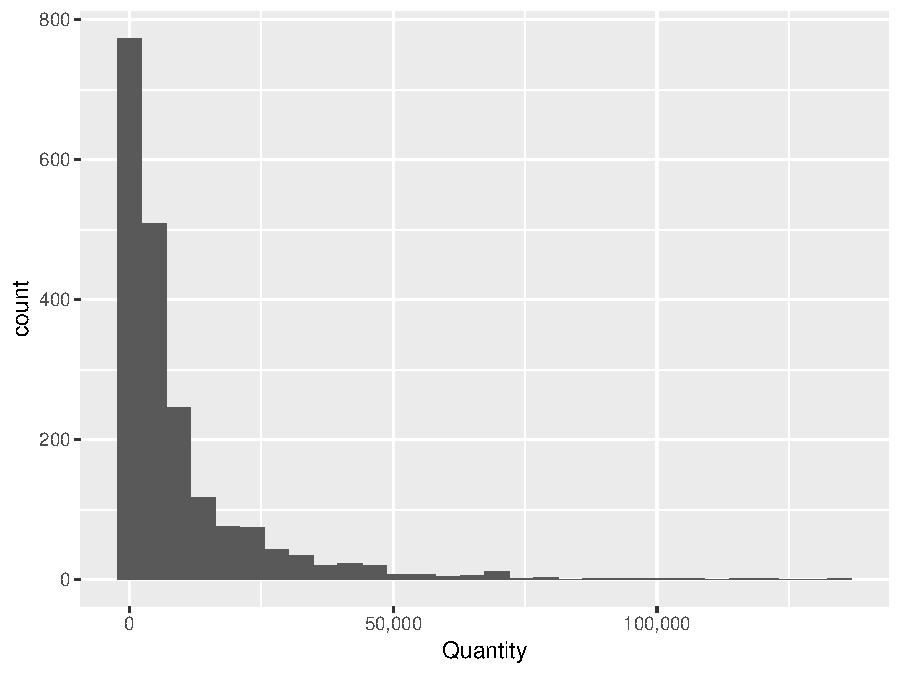
\includegraphics{UChicago-MScA-Capstone_files/figure-latex/Quantity_Histogram-1.pdf}
\caption{(\#fig:Quantity\_Histogram)Histogram of Quantity}
\end{figure}
\subsection{Distribution of Quantity over
time}\label{distribution-of-quantity-over-time}

The figure below breaks down shipments over time. There is a large
degree of seasonal behavior. Tomato bag sales increase during summer
time from June to August and begin to drop off in September and October.
Quantity is very small during other months of the year.
\begin{figure}
\centering
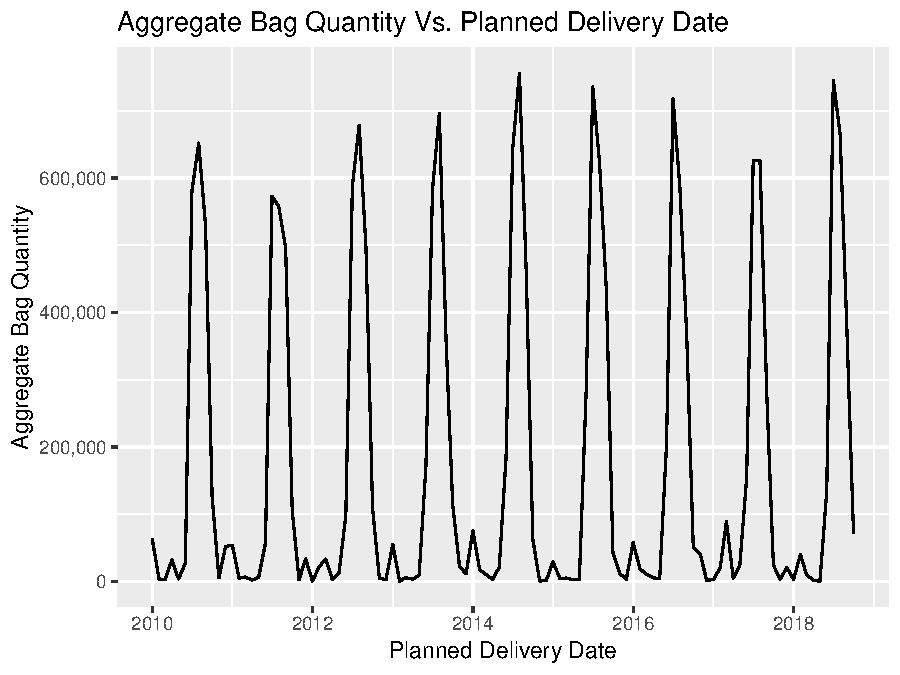
\includegraphics{UChicago-MScA-Capstone_files/figure-latex/Quantity_Time-1.pdf}
\caption{(\#fig:Quantity\_Time)Quantity over Time}
\end{figure}
\subsection{Distribution of Quantity over
Time}\label{distribution-of-quantity-over-time-1}

The figure below breaks down shipments over time. There is a large
degree of seasonal behavior. Tomato bag sales increase during summer
time from June to August and begin to drop off in September and October.
Quantity is very small during other months of the year.
\begin{figure}
\centering
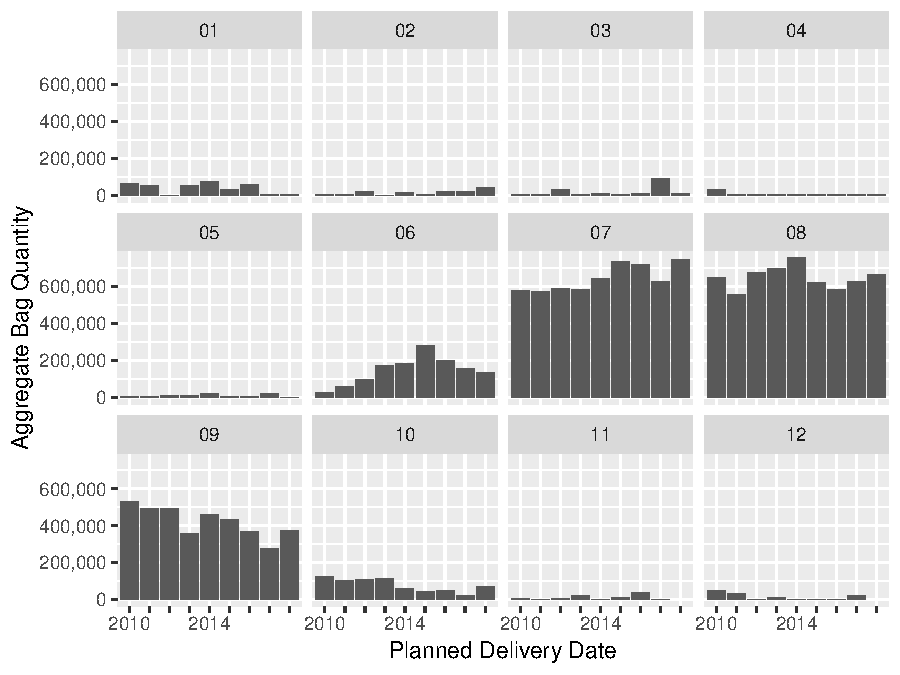
\includegraphics{UChicago-MScA-Capstone_files/figure-latex/Quantity_Month-1.pdf}
\caption{(\#fig:Quantity\_Month)Monthy Quantity by Year}
\end{figure}
\subsection{Quantity by Item Number}\label{quantity-by-item-number}

In the figure below, total order quantity are aggregated by item number
and then ordered by descending total quantity. Over 86\% of bag
quantities are driven by the top 10 out of a total of 60 item numbers.
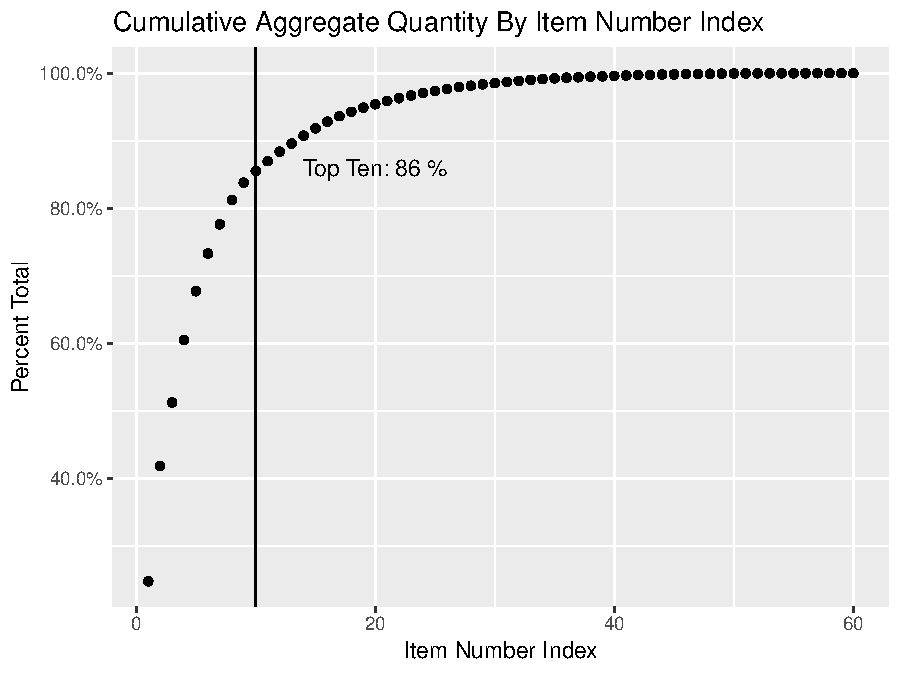
\includegraphics{UChicago-MScA-Capstone_files/figure-latex/IN_cumulative-1.pdf}

\subsection{Quantity by Top Business
Partner}\label{quantity-by-top-business-partner}

The figure below aggregates quantity by item number and then orders
quantity descendingly. It suggests that over 93\% of bag quantities are
driven by the top 10 out of the 23 top business partners.
\begin{figure}
\centering
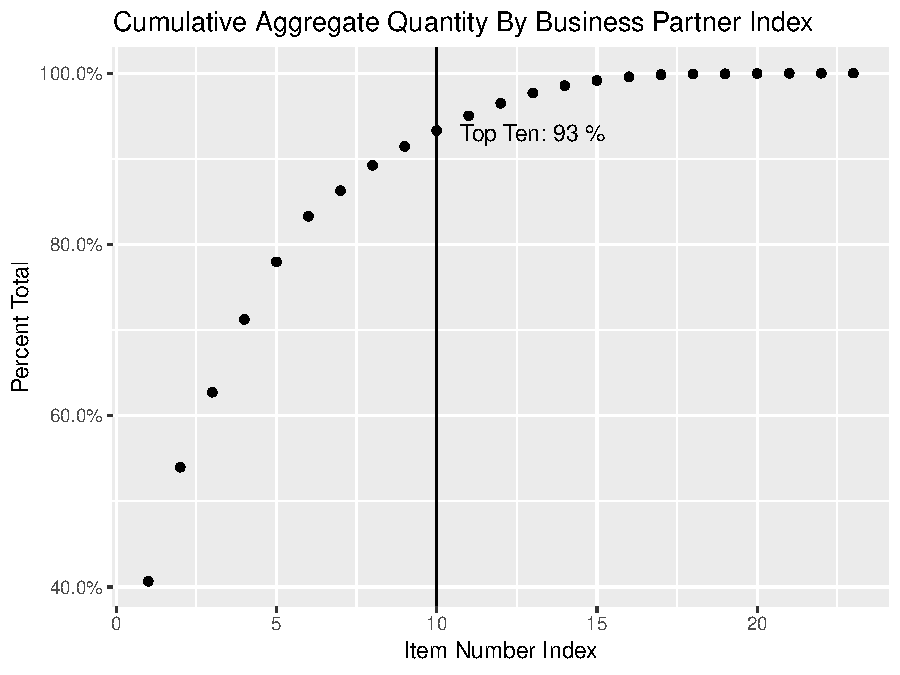
\includegraphics{UChicago-MScA-Capstone_files/figure-latex/BP_Cumulative-1.pdf}
\caption{(\#fig:BP\_Cumulative)Cumulative Sales by Business Partner}
\end{figure}
\subsection{External Data Collection}\label{external-data-collection}

We collected Social Media data from two sources: Twitter and the Google
Trends. Google Trends summarised US monthly search statistics from 2004
to 2019. The twitter data collected are of US users from 2007 to 2018.

Google Trends returns a single value showing how frequently a given
search term (e.g. `Tomato') goes in Google's search engine relative to
its total search frequency for a given period.

Twitter data were gathered by collecting relevant tweets from Twitter
using key search words as shown in Table \_\_ below. We can grab a tweet
based on defined keyword from Twitter by calling the Twitter API
function. Subsequently, we can categorize opinions expressed in a piece
of text, in order to determine opinion on our research (i.e, positive,
negative, or neutral).
\begin{verbatim}

Attaching package: 'kableExtra'
\end{verbatim}
\begin{verbatim}
The following object is masked from 'package:dplyr':

    group_rows
\end{verbatim}
\begin{longtable}[]{@{}rrrrr@{}}
\toprule
External Data Source & Frequency Granularity & Range & Size & Data
Type\tabularnewline
\midrule
\endhead
Google Trend & Monthly & 2004-2019 & 182 & Numeric\tabularnewline
Twitter & Monthly & 2007-2019 & & Text, Numeric\tabularnewline
\bottomrule
\end{longtable}
Table \_\_ above shows the description of the social media dataset. The
google trend dataset based on relative search frequency is on a monthly
basis. The monthly dataset at the time of reporting has 182 rows.

The Twitter data are sampled via a quasi-random approach that grabs data
monthly over the entire period of 2007 - 2018. We had to employ this
method of querying due to the nature of the Twitter API and its
restrictions on total tweets returned. The Twitter API returns tweets in
reverse chronological order. The total number of tweets that would
mention one of our keywords would be vastly larger than the number we
could collect over the course of our data collection period (January
2019 - March 2019). Limited in this way, we decided to strategically
collect tweets from each month of the year between January 2007 and
March 2019.

\textbf{Assumptions \& Limitation}

Google Trends Assumptions We limited the Google Trends search to the
United States. The keywords are independent of each other.

Limitation: The actual number of searches for the term being queried is
not made available. Instead, the data are reported from 0-100, where 100
represents the maximum relative search frequency.

Resolution: Each term selected will be queried individually.

\textbf{Twitter Datasets} Assumptions We limited Twitter data to the
United States. The frequency of tweets we collected for each keyword
will be independent of the time period in which we collected them.

Limitations The demographic information of the twitter account user
cannot be determined. With the limitation of our premium account API
activity, we can only submit 100 requests to collect tweet per month.
Per each request, we can get a maximum of 500 tweets back. The language
associated with the Twitter account returned from the API does not
guarantee the language of the Tweet. While we specified English language
tweets, we received many tweets that were not in English. We
subsequently dropped these tweets.

\textbf{Plan for use}

Twitter data We developed a sentiment index for all tweets using natural
language processing techniques tilizing the textblob Library to analyze
how similar or discrepant the meaning of tweets among each keyword

Google Trends Correlation analysis of frequency of individual search
terms compared to quantity Subsequent seasonality \& trend analysis to
identify meaningful predictors

Twitter Data

We have collected tweets based on the keywords in Table 3 below. Tweets
were aggregated on a monthly basis. The figure below shows how
frequently the keywords appears in the returned tweets over time. Pizza
is more frequently mentioned in Twitter than other keywords.

Google Trend Analysis

We collected Google Trend data consisting the same keywords as we did in
Tweet collection. The Google Trends data was standardized and
subsequently the cross correlation was found with respect to the Scholle
bag sales. Figure \_\_ displays the results of the cross correlation
analysis.
\begin{figure}
\centering
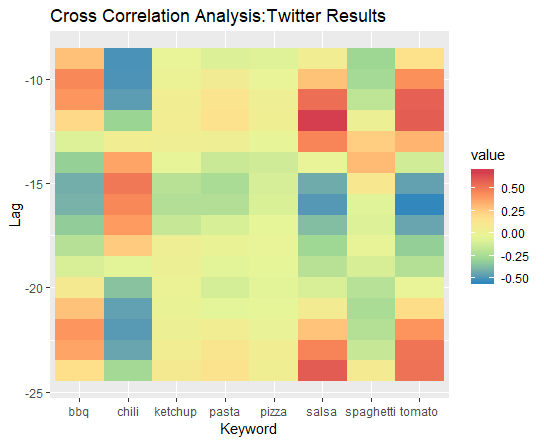
\includegraphics{./figure/CCF_Results_Google.png}
\caption{CCF Google}
\end{figure}
\begin{longtable}[]{@{}rrrrrrrr@{}}
\toprule
bbq & chili & ketchup & pasta & pizza & salsa & spaghetti &
tomato\tabularnewline
\midrule
\endhead
Lag 10 & Lag 15 & None & None & None & Lag 12 & None & Lag
12\tabularnewline
\bottomrule
\end{longtable}
In Table 4 above, we highlight cross-correlations greater than 0.5 and
with a time period of greater than 8 months. Since the Scholle bag sales
data are records of the demand are placed well in advance of the desired
delivery date, we would expect a long lag window in order for the trends
of social media to drive market forces that would affect demand. Red
indicates positive relations and blue indicates negative correlations.
The deeper the color, the greater its correlation with Scholle's data.

\subsection*{Tweet Sentiment Analysis}\label{tweet-sentiment-analysis}
\addcontentsline{toc}{subsection}{Tweet Sentiment Analysis}

We have conducted the following steps to conduct the sentiment analysis
of the tweets.

\textbf{Text Cleanup Pipeline:} 1. Remove RT, URLs and non-text
characters (except @ and punctuation symbols) 2. Handle mentions by
replacing with upper case letters. 3. Remove all remaining non-text
characters (including @ symbol and excluding punctuation symbols). 4.
Check the language of the cleaned up tweet and drop any tweets that are
not in English.

\textbf{SpaCy Pipeline:}

We used the spaCy English Core Web Large model to analyze each tweet to
process into three data sets: 1. Tokenization - each tweet was broken
into its component elements of words, punctuation, etc. 2. Dependency
Parsing - Annotate the tweet to add the syntactic dependency within the
tweet i.e.~compare link verbs to their respective nouns. 3. Named
Entities - Each tweet was analyzed to identify the named entities in the
tweet. These entities will include the mentions because they were
capitalized in the Text Cleanup Pipeline. 4. Removal of stop words - all
stop words identified were removed.

\textbf{Vector Extraction:}

Spacy includes vector representations for individual words as well as
entire entire sentences. See Figure 22 below for the Keyword Distance
using Spacy.These are represented as 300 dimension Numpy arrays. To
begin, we confirmed that were was a reasonable cosine distance measure
between each of the keywords.
\begin{figure}
\centering
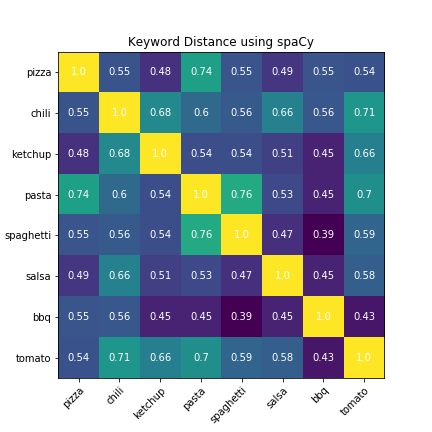
\includegraphics{./figure/Keyword_Distance_Spacy.png}
\caption{Spacy Keyword Distance}
\end{figure}
There is a reasonable distance between each of the keywords with the
exception of bbq and barbecue but this is to be expected since they
reference the same thing.

In addition, vectors representations of each tweet can be extracted. For
each tweet keyword we summarised all vectors by finding their mean
values for each dimension. We then found the pairwise distance measures
for these `average' tweets. See in the figure below
\begin{figure}
\centering
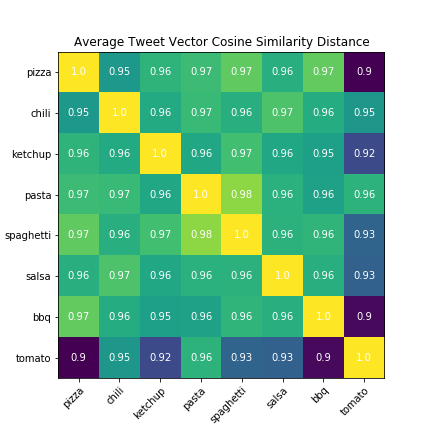
\includegraphics{./figure/Tweet_Distance_Spacy.png}
\caption{Spacy Mean Vector Distance}
\end{figure}
Here, the ``average'' tweets are rather similar to each other with the
greatest distance from tomato to salsa.

In future work we will leverage these vector representations of the
tweets to conduct transfer learning to identify tweet sentiment.

\textbf{Sentiment Analysis using TextBlob}

TextBlob is an open source Python library for conducting natural
language processing. It has a built in sentiment analyzer that utilizes
two axes of analysis Polarity and Subjectivity. Polarity refers to a
positive or negative sentiment and ranges from positive one to negative
one respectively. Subjective expresses the subjectivity or objectivity
of the text. See Figure 24 below for the Tweet Polarity. The
subjectivity axis ranges from zero to positive one where 0 is very
objective and 1 is very subjective. See Figure 25 below for the Tweet
Subjectivity .
\begin{figure}
\centering
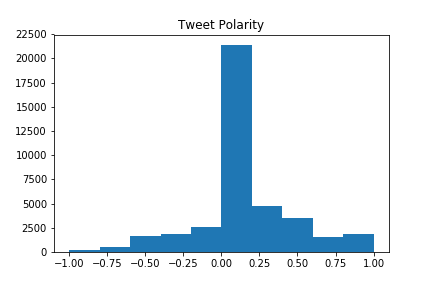
\includegraphics{./figure/Tweet_Polarity.png}
\caption{Tweet Polarity}
\end{figure}
\begin{figure}
\centering
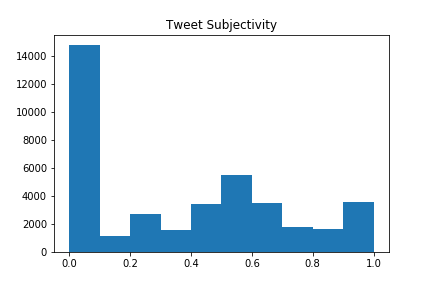
\includegraphics{./figure/Tweet_Subjectivity.png}
\caption{Tweet Subjectivity}
\end{figure}
\begin{figure}
\centering
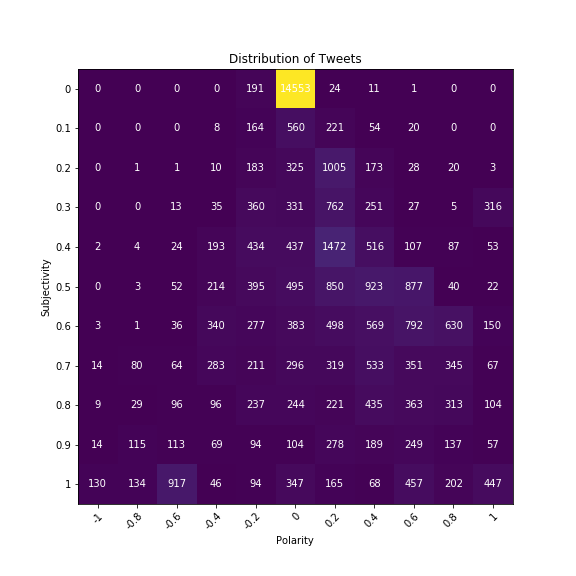
\includegraphics{./figure/Tweet_Distribution.png}
\caption{Tweet Distribution}
\end{figure}
TextBlob categorizes the vast majority of tweets as non-subjective
non-polar.

With the tweets collected, we generated a sentiment index by taking each
tweet's subjectivity \& polarity and multiplied them by the retweet
count for that tweet. We then aggregated the sentiment index at the
monthly level for each keyword. The cross correlation between the
Scholle data and the sentiment monthly index for the overall sentiment
and for each keyword was calculated and the results displayed in the
figure below.
\begin{figure}
\centering
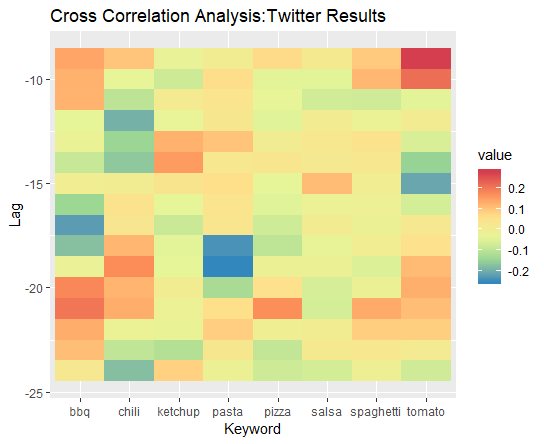
\includegraphics{./figure/CCF_Twitter_Results.png}
\caption{Twitter CCF}
\end{figure}
It is important to note the difference in scale relative to the Google
Trends results; the correlations to the Twitter sentiment index are much
weaker.

The table below compiles the list of lagged values used in our analysis.
\begin{longtable}[]{@{}rrrrrrrr@{}}
\toprule
bbq & chili & ketchup & pasta & pizza & salsa & spaghetti &
tomato\tabularnewline
\midrule
\endhead
Lag 17 & None & None & Lag 18 & None & None & None & Lag
15\tabularnewline
\bottomrule
\end{longtable}
\subsection*{Model Selection Metrics}\label{model-selection-metrics}
\addcontentsline{toc}{subsection}{Model Selection Metrics}

Selection of Metrics

In order to determine the best model, we began by choosing selection
metrics to test each model against. The following metrics outlined below
will be used to measure the performance of each model. 1. SMAPE 2. RMSE
3. \% bias -- no of time above forecast vs below. 4. Accuracy

\textbf{sMAPE -Symmetric Mean Absolute Percentage Error}

Symmetric mean absolute percentage error (sMAPE) is an accuracy measure
based on percentage (or relative) errors. It allows us to understand
error independent of scale.

\[sMAPE=\frac{100\%}{n}\frac{|A_t-F_t|}{(|A_t|+|F_t|)/2}\]

sMAPE has a lower bound of 0\% and an upper bound of 100\%. The best
value will be 0\% while the worst value will be 100\%.

The major limitation with sMAPE is that it gives more penalties to
underestimates than overestimates.

\textbf{RMSE- Root Mean Squared Error}

The root mean squared error (RMSE) of an estimator measures the average
of the squares of the errors---that is, the average squared difference
between the estimated values and what is estimated. The square root of
this value is then taken to produce the RMSE.

\[RMSE = \sqrt{\frac{\sum^n(A_t-F_t)^2}{n}}\]

RMSE measures the variation between predicted and measured values and it
provides us a basis for measuring the model variance on the same scale
as the data.

The RMSE is a measure of the quality of an estimator. RMSE is always
non-negative, as the process of squaring removes any negative signs. It
also penalizes larger differences. The best value is zero while the
worst value is unbounded.

In sum, the lower the RMSE, the smaller the error, the better the
estimator.

\textbf{Percent Bias -- ratio of model high or low.}

Bias refers to the propensity of a measurement process to over- or
under-estimate the value of a population parameter. Percent bias (PBIAS)
measures the average tendency of the predicted values to be larger or
smaller than the actual values.

Percent Bias is calculated by taking the sign of the residual for each
data point and setting positive values to 1 and negatives values to
zero. These are then averaged and multiplied by 100 to produce a
percentage. The best percentage bias is 50\% - there are just as many
over predictions as under predictions. The worst percentage bias is
either 0\% or 100\% as the model is regularly over- or under-estimating
the actual data.

\textbf{Accuracy - Mean Accuracy between Model \& Actual}

Accuracy measures the closeness of a model prediction to the actual
value. In our case we are measuring the mean accuracy for all model
predictions versus actual values. The best accuracy measure is 1; the
prediction and the actual are the same so their ratio is 1. Accuracies
that diverge from 1 are bad; a value greater than 1 means the prediction
was higher than the actual while a value below 1 is means the
predictions was lower than the actual. We aggregate the accuracy measure
for each data point and find the overall mean. One precaution to
consider by using this procedure is it may mask an underlying trend in
prediction of the accuracy in which the model could overestimate early
and then underestimate late or other non-linear behavior.

\textbf{Training and Forecasting Windows}

In order to evaluate our model to avoid either overfitting or
underfitting , we split our dataset into a training set and a test set.
Based on our discussions with Scholle, the test set will be the
subsequent 18 months. The length of the training period was chosen based
on the evaluation of the model stability of our baseline model using a
rolling window cross validation.

\textbf{Rolling Window Cross Validation}

Time series data present a unique challenge in analysis in that the data
are not independent - they are collected at regular intervals over the
course of time. We employed rolling window cross validation to generate
multiple train and test sets from the overall data set. Initially we
explored the model stability of our baseline model and used the best
criteria from that in order to decide the length of the cross validation
window.

Because of the highly seasonal nature of the data, we created a baseline
model using only Scholle data. We used periods of 2-year, 4-year and
6-year windows, to identify the forecast window period with the greatest
stability.

\section*{Results of model performance and
validation}\label{results-of-model-performance-and-validation}
\addcontentsline{toc}{section}{Results of model performance and
validation}

\subsection*{Baseline Model - Prophet}\label{baseline-model---prophet}
\addcontentsline{toc}{subsection}{Baseline Model - Prophet}

Prophet is an open-source tool developed by Facebook to conduct time
series modeling. Prophet models data using a decomposable time series
model with three main components: trend, seasonality, and holidays. The
focus is to model the time series via regression instead of as a
generative model like ARIMA would. This is done for flexibility, the
ability to handle irregularly spaced data, speed, and interpretability.

\textbf{Cross-Validation Window Selection}

The figures below show results of the cross-validation analysis at 2, 4
and 6 year training windows using the Prophet Model.
\begin{figure}
\centering
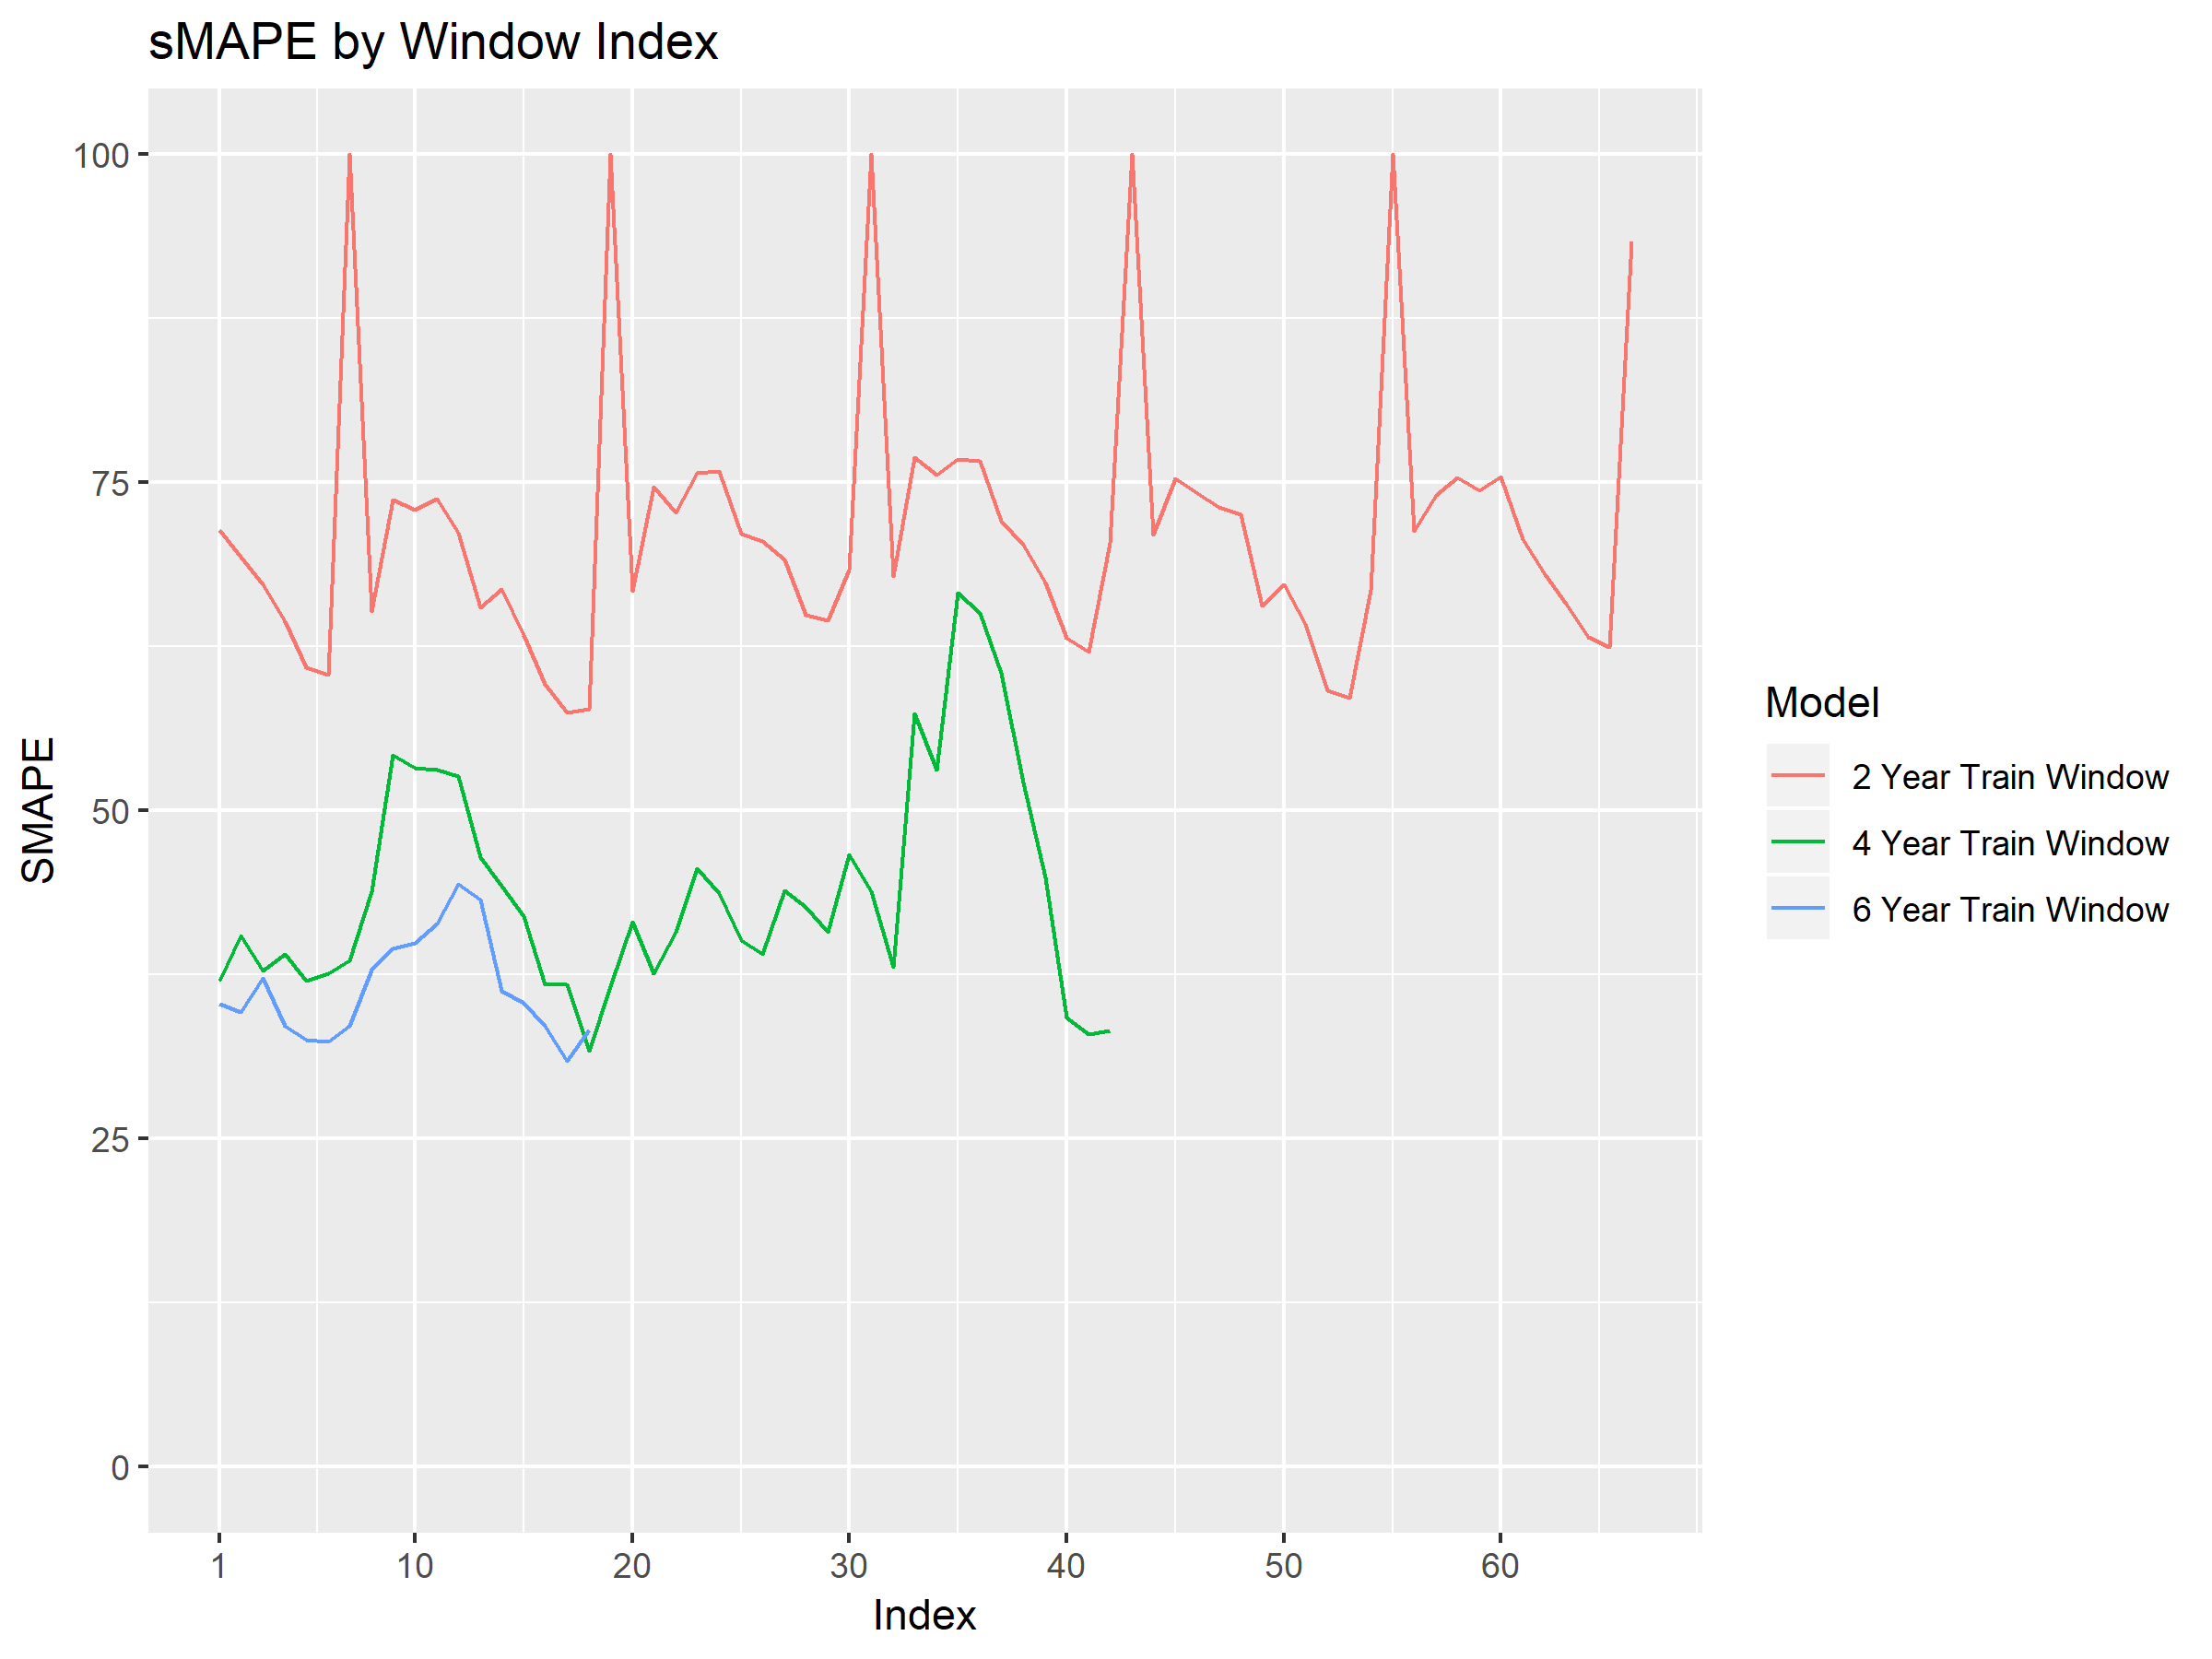
\includegraphics{./figure/Prophet_SMAPE_CV.png}
\caption{sMAPE CV Window Selection}
\end{figure}
\begin{figure}
\centering
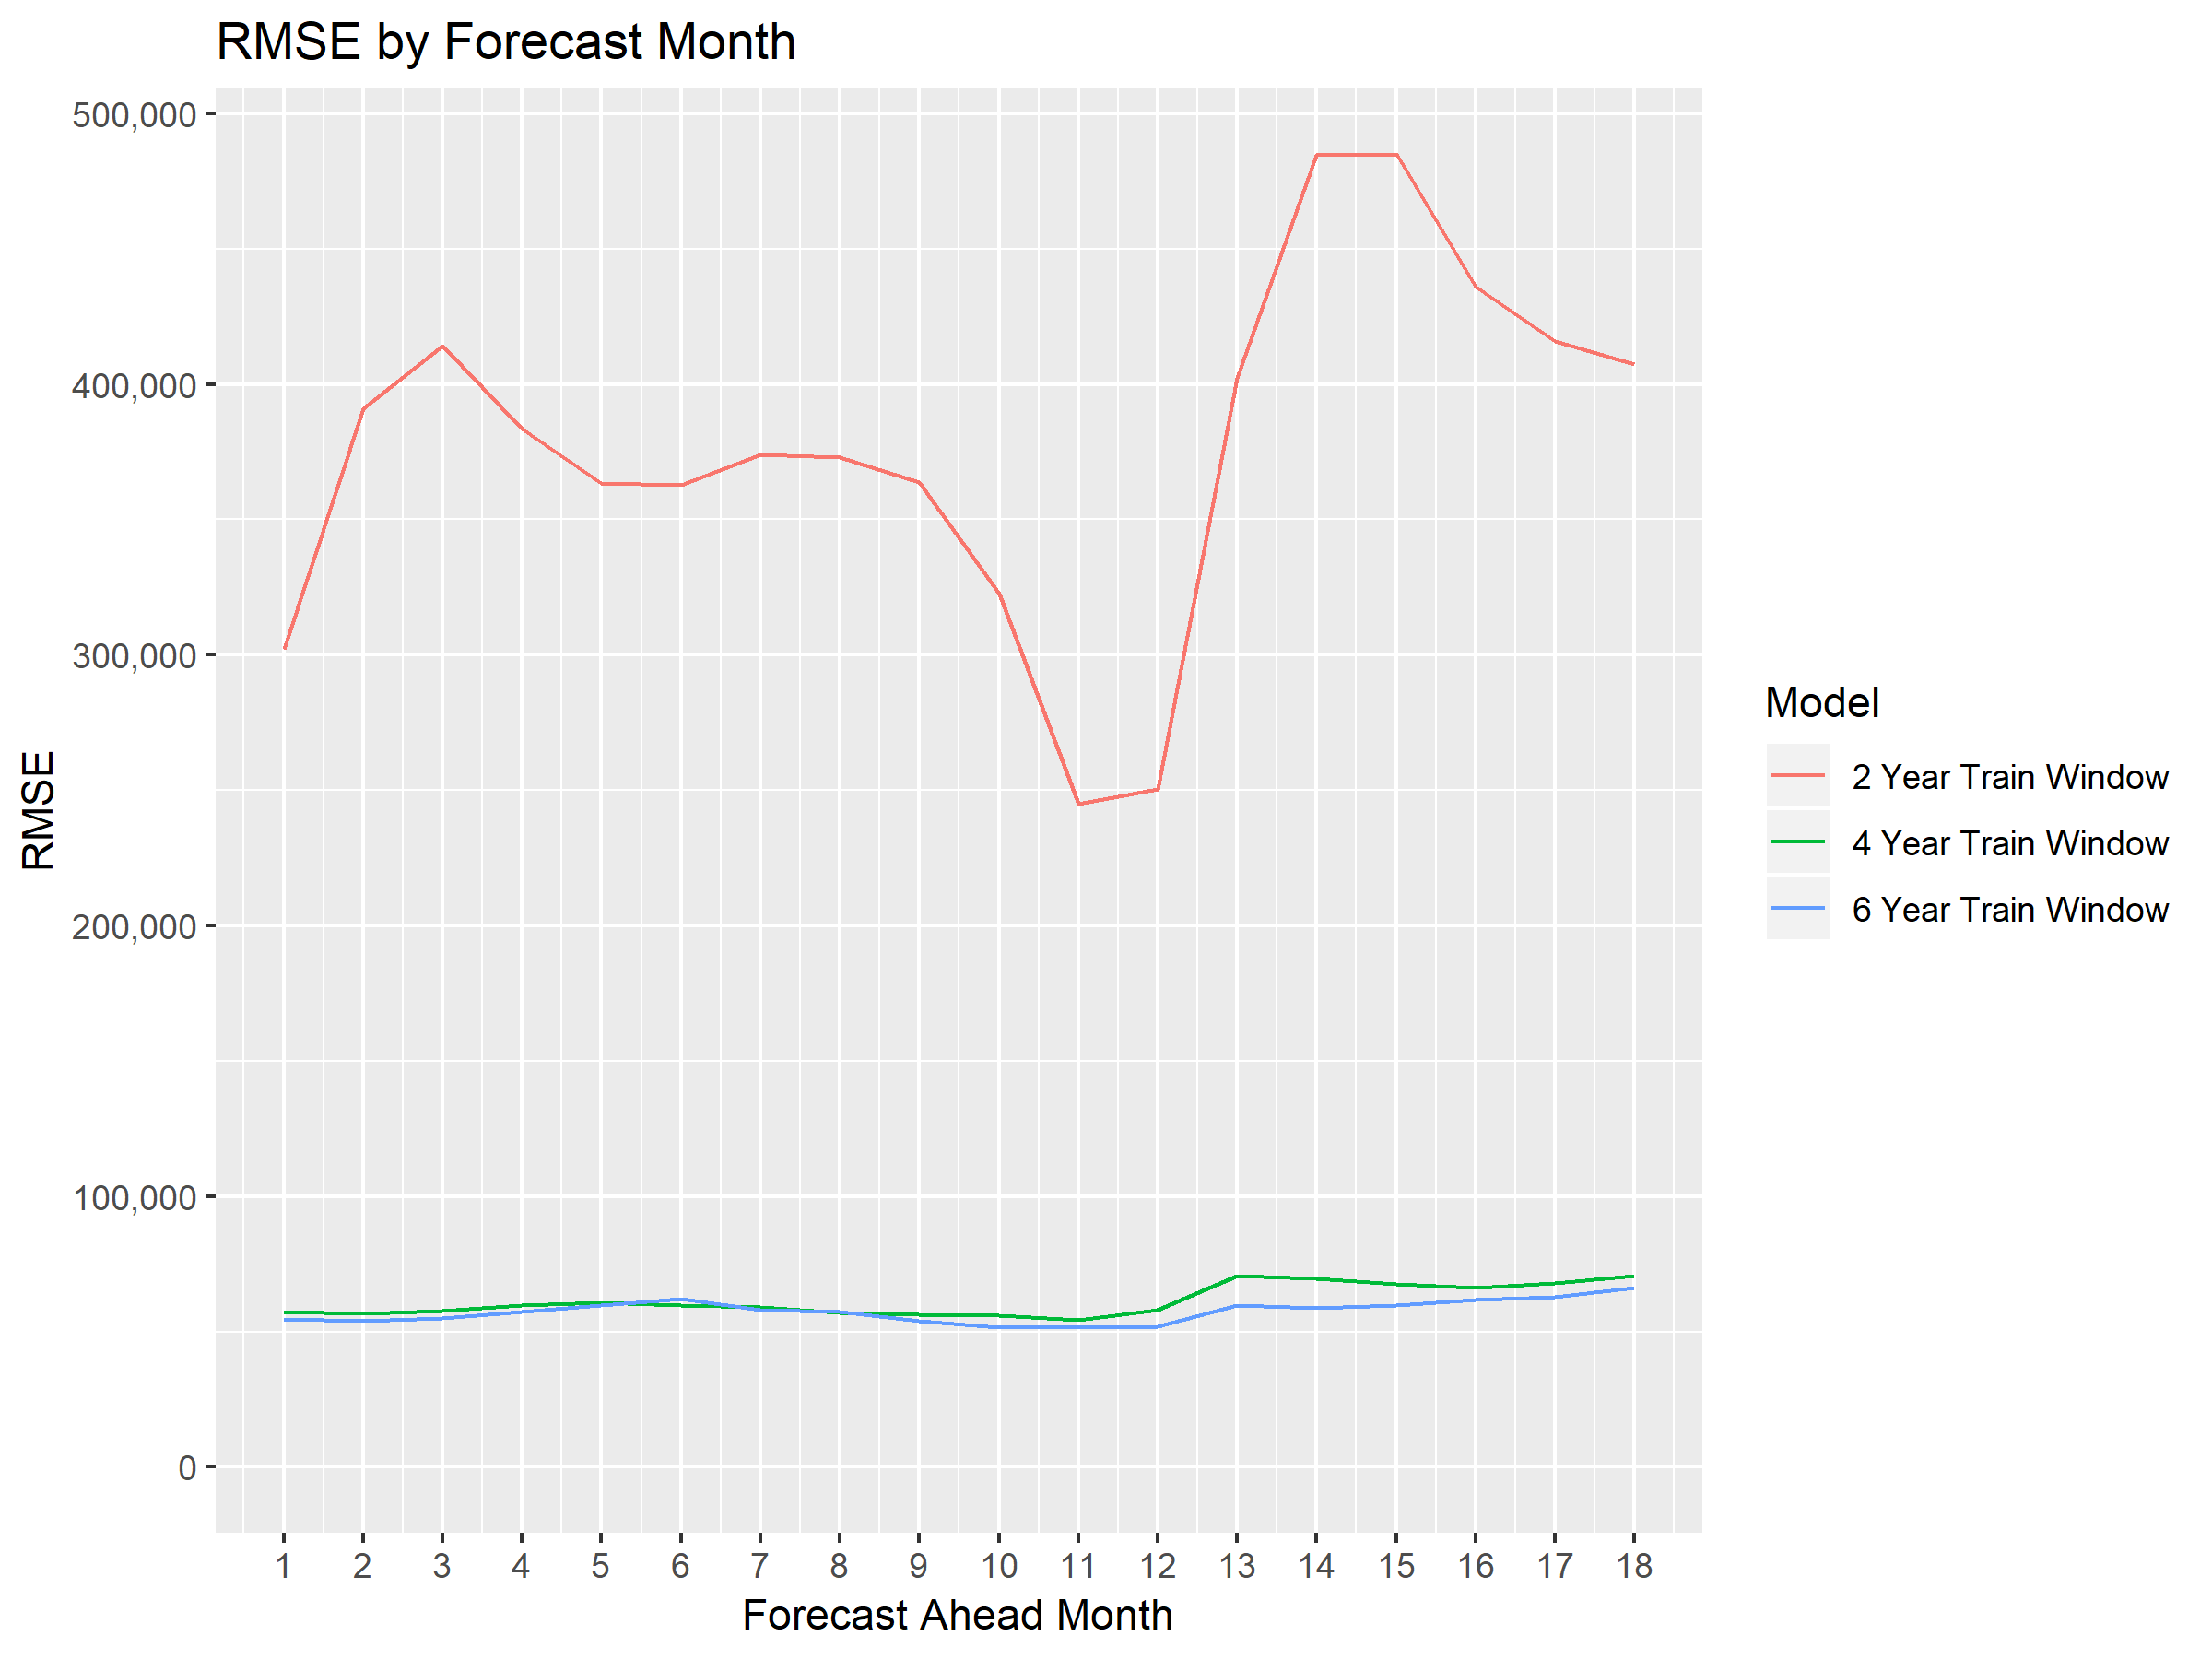
\includegraphics{./figure/Prophet_RMSE_CV.png}
\caption{RMSE CV Window Selection}
\end{figure}
For both sMAPE and RMSE, the 2 year window shows much higher variability
than the 4 or 6 year windows. Given the similarity of the 4 and 6 year
windows RMSE, we chose the 4 year window to both reduce the data
requirements of the model and allow for additional cross-validation of
each other model. A 4 year cross validation allows us to generate 42
complete training and testing windows whereas A 6 year cross validation
window only allows us to generate 18.

\textbf{Baseline Model Results}

The reported model metrics are the mean values for each of the cross
validation periods collected.
\begin{longtable}[]{@{}rrrrr@{}}
\toprule
X & sMAPE & RMSE & X..Bias & Accuracy\tabularnewline
\midrule
\endhead
Train & 30\% & 29896.68 & 22\% & 0.86\tabularnewline
Test & 43\% & 62625.69 & 67\% & 4.04\tabularnewline
\bottomrule
\end{longtable}
\subsection*{Challenger Model sARIMA}\label{challenger-model-sarima}
\addcontentsline{toc}{subsection}{Challenger Model sARIMA}

Seasonality is a key feature of the dataset, as it was observed that the
Tomato bags sales increase significantly during summer time from June to
August and drop in September and October while repeating this cycle
annually.This key attributes in the dataset meant we deploy a model that
uses differencing at a lag equalling the number of seasons to remove
additive seasonal effect.

For this challenger, we split the data into two groupings; harvest
months (June -October) and all months. In the Table 7 \& 8 below, we
summarise the result for the model:
\begin{longtable}[]{@{}rrrrr@{}}
\toprule
X & sMAPE & RMSE & X..Bias & Accuracy\tabularnewline
\midrule
\endhead
Train & 9\% & 125522.0 & 19\% & 1.76\tabularnewline
Test & 68\% & 338725.3 & 100\% & 0.43\tabularnewline
\bottomrule
\end{longtable}
In the figure below, the mean forecast value is highlighted in blue and
the actual value is captured in red, and the confidence interval ranging
between 80\%-95\%. The actual values are represented in black.
\begin{figure}
\centering
\includegraphics{./figure/Arima_12month.png}
\caption{Arima(0,0,2)(0,1,1)12 with Drift}
\end{figure}
\begin{figure}
\centering
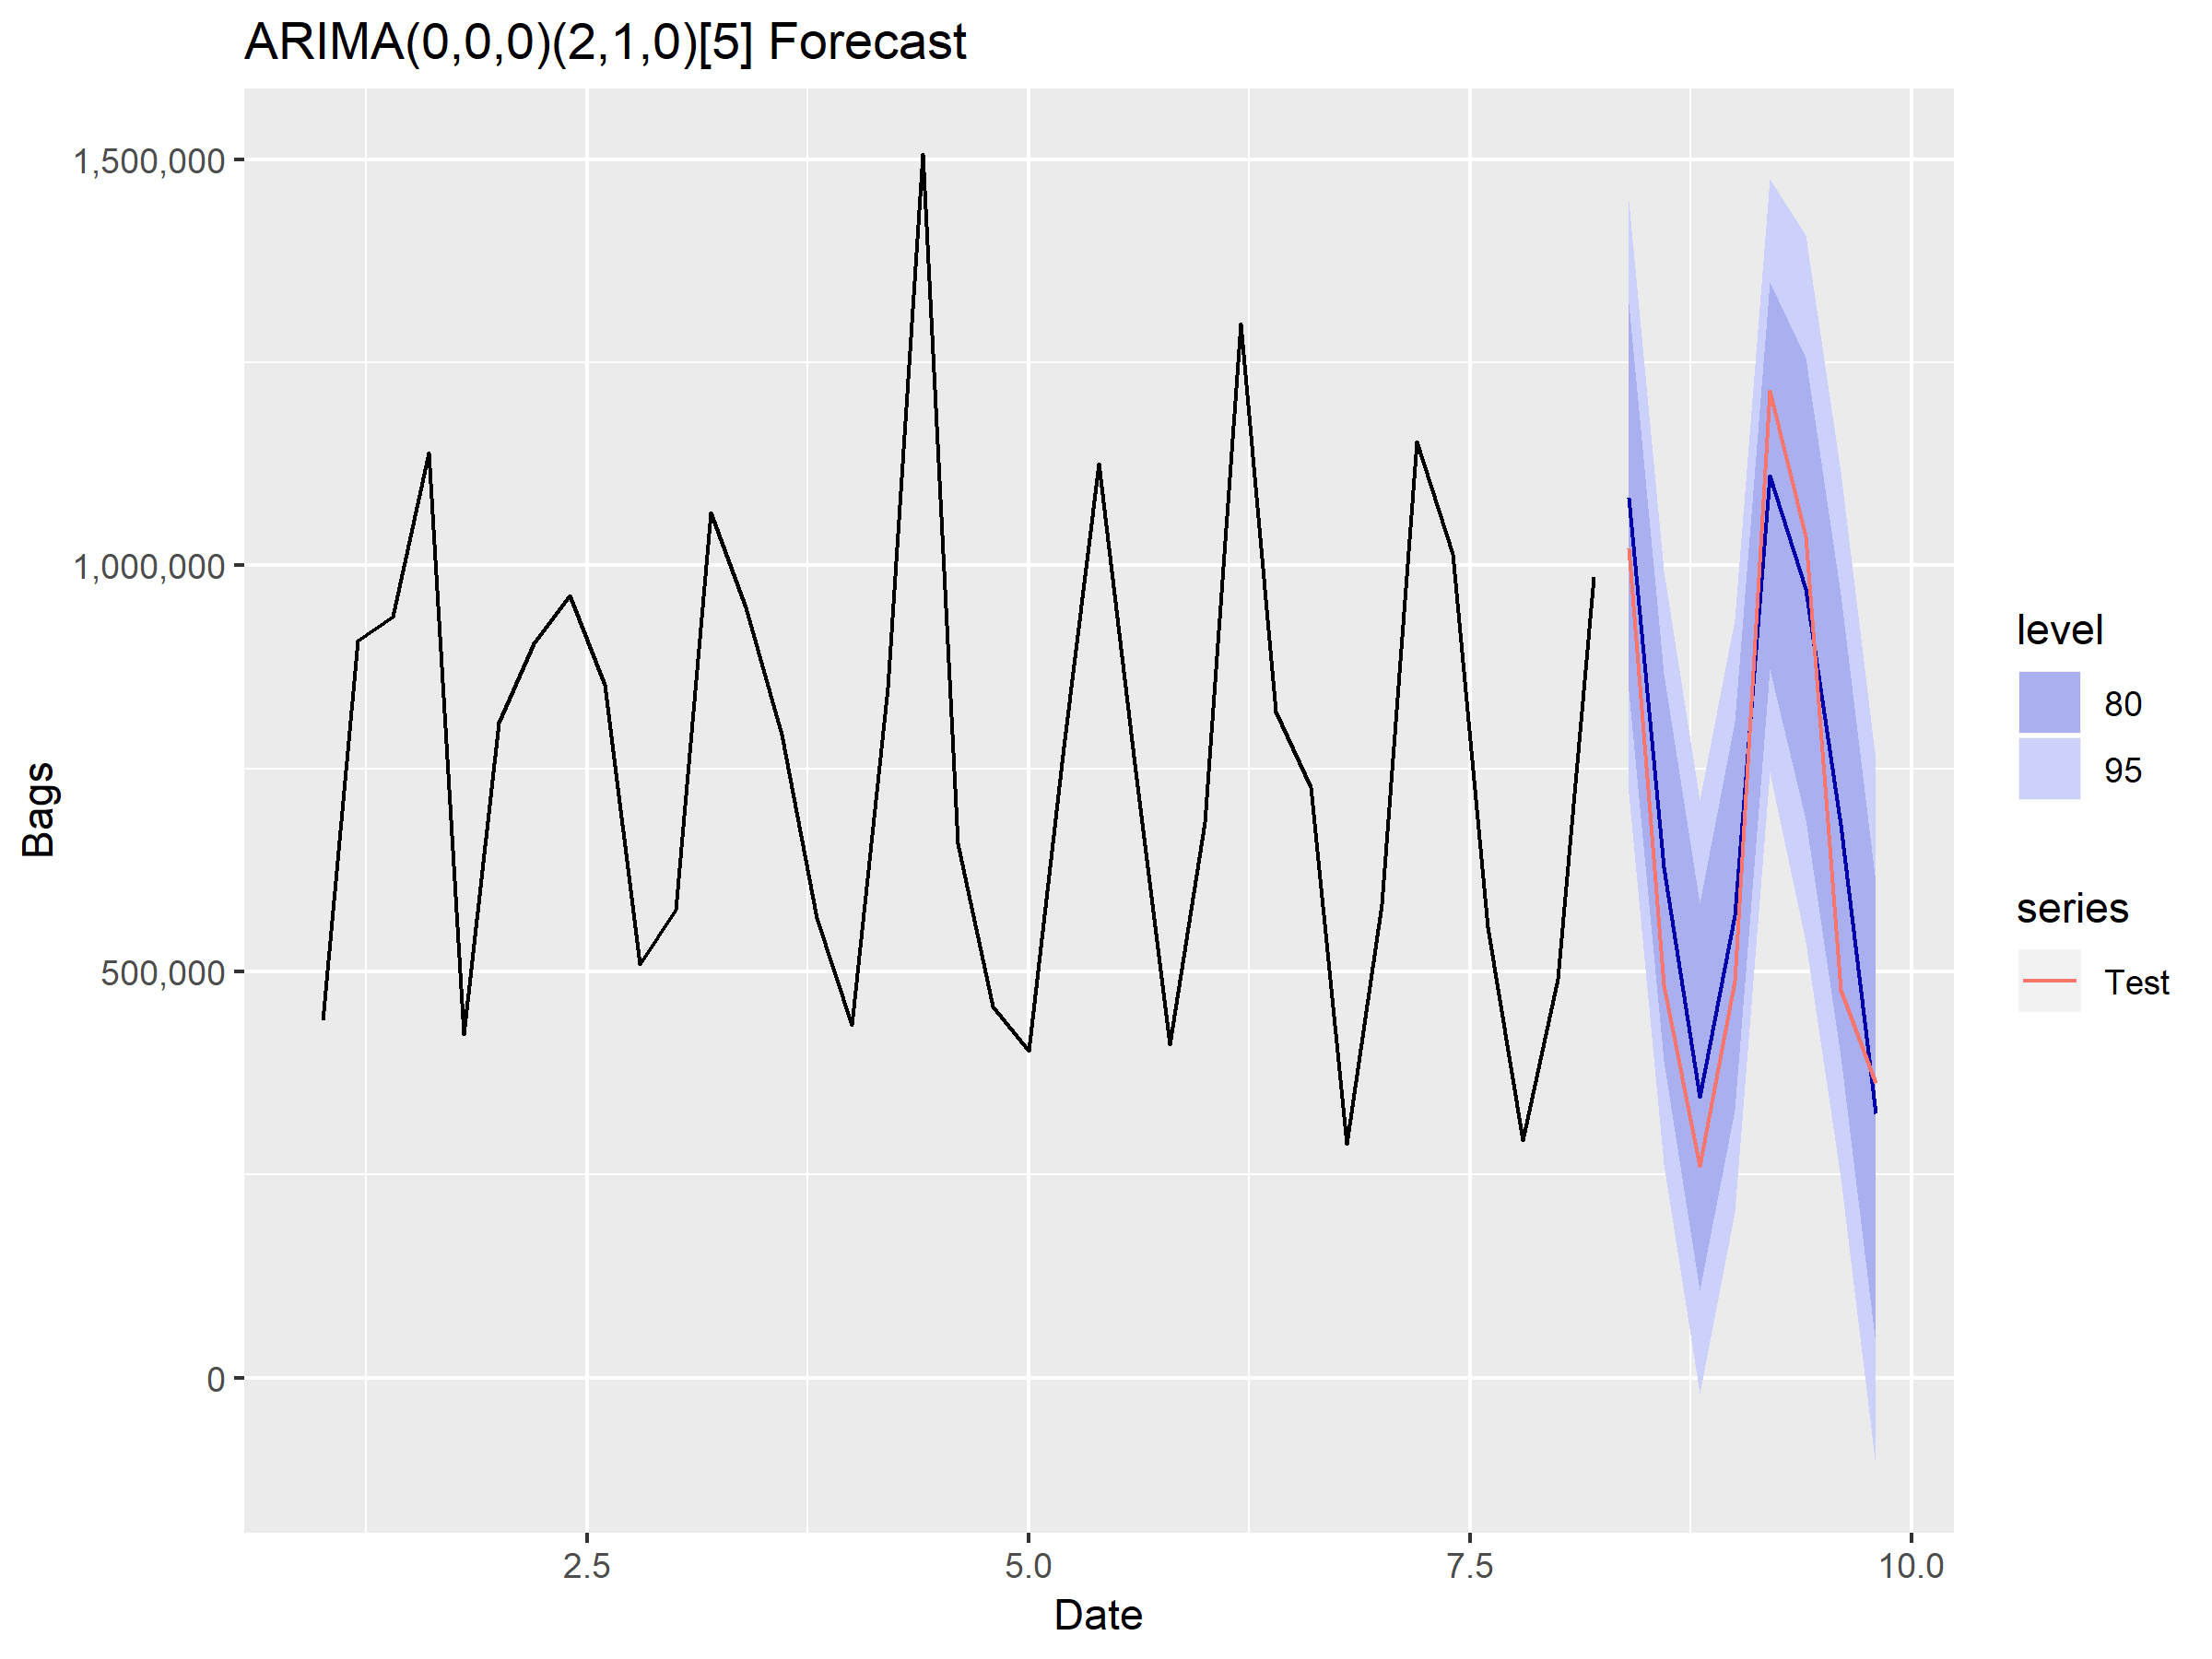
\includegraphics{./figure/HarvestArima.png}
\caption{Arima(0,0,0)(2,1,0)5}
\end{figure}
\subsection{Challenger Model - Regression with ARIMA Errors\#\#\#
\{unnumbered\}}\label{challenger-model---regression-with-arima-errors-unnumbered}

The first challenger model we built is regression model with ARIMA
errors. While the regression model allows for the inclusion of predictor
variables, it does not allow for the subtle time series dynamics that
can be handled with ARIMA models. The regression with ARIMA errors model
solves this problem by fitting regression models with all the relevant
variables first, and then applying ARIMA to the residuals of the
regression to detect time series elements in the residuals.

We explored the correlations of twitter data and Google trend Scholle
tomato bag sales and found the keywords and lags in Table 4 and Table 6
tend to strongly correlated with tomato bag sales. Since the regression
with ARIMA errors is based on linear regression, we first build a linear
regression model these keywords and lags. Results are shown in below
Table 10. Significant variables are highlighted in green.

Based on the variables significant in the linear model, we built the
regression model with ARIMA errors. The parameters and accuracy are
shown below in Table 11 and Table 12.
\begin{longtable}[]{@{}rrr@{}}
\toprule
Keyword\ldots{}Lag & Estimate & P.Value\tabularnewline
\midrule
\endhead
Google bbq lag 10 & -39516 & 0.137173\tabularnewline
Google chili lag 15 & -42963 & 0.017008\tabularnewline
Google salsa lag 12 & 92606 & 0.000366\tabularnewline
Google tomato lag 12 & 122522 & 0.000145\tabularnewline
\bottomrule
\end{longtable}
Based on the variables significant in the linear model, we built the
regression model with ARIMA errors. The parameters and accuracy are
shown below in Table and Table 12.
\begin{longtable}[]{@{}rrr@{}}
\toprule
Keyword\ldots{}Lag & Estimate & P.Value\tabularnewline
\midrule
\endhead
Google bbq lag 10 & -39516 & 0.137173\tabularnewline
Google chili lag 15 & -42963 & 0.017008\tabularnewline
Google salsa lag 12 & 92606 & 0.000366\tabularnewline
Google tomato lag 12 & 122522 & 0.000145\tabularnewline
\bottomrule
\end{longtable}
Positive coefficients imply that for a unit increase in the variable,
there is a corresponding positive increase in the Scholle bag sales.
Negative coefficients imply that for a unit increase in the variable,
there is a corresponding negative decrease in the Scholle bag sales.The
negative coefficient shows there is an inverse relationship between the
variable and Scholle bag sales.
\begin{longtable}[]{@{}rrrrr@{}}
\toprule
X & sMAPE & RMSE & X..Bias & Accuracy\tabularnewline
\midrule
\endhead
Train & 25\% & 93857.76 & 20\% & 0.38\tabularnewline
Test & 44\% & 68342.19 & 58\% & -0.93\tabularnewline
\bottomrule
\end{longtable}
The above results indicate that Google trend data tend to have a greater
influence in the predictions than twitter data, because the count in
google searches is more direct in measuring the importance of the
keywords and lags, compared to twitter data which might lose some
information both due to the limitations in gathering tweet data and due
to the complicated natural language preprocessing process. The ARIMA
errors is (0,0,0), indicating our model has extracting enough
informations and there's no time series dynamics in the residuals.

\subsection*{Challenger Model - Random Forest
Regression}\label{challenger-model---random-forest-regression}
\addcontentsline{toc}{subsection}{Challenger Model - Random Forest
Regression}

The second challenger model we built was a Random Forest Regression
Model. Random Forest leverages many regression trees to build a
consensus model in addition to bootstrap aggregation or bagging to
generate additional augmented data. Bagging simply builds additional
training sets by sampling with replacement from provided training data.
Each individual tree uses the bagged training data and selects a random
subset of features at each branching point rather than all features
available to build the regression. This restriction forces the model to
create a more robust estimator.

One useful feature when using tree-based approaches for regression is
the ability to use categorical or ordinal predictors without the need
for one-hot-encoding. In our model we represented the date as a pair of
categorical variables, one for year and a second for month. We chose to
do this because of the seasonal nature of the data.

In addition, we decided to challenge the model by only using lags that
we thought to be have a reasonable explanation for their effect. To this
end we chose to use lags greater than 9 months. Our logic was that it
would take time for an increase or decrease in the social media presence
of one of the keywords selected to go from an uptick in interest of
consumer products to be captured by Scholle's bag sales.

The table below displays the results of our Random Forest model.
\begin{longtable}[]{@{}rrrrr@{}}
\toprule
X & sMAPE & RMSE & X..Bias & Accuracy\tabularnewline
\midrule
\endhead
Train & 38\% & 66560.6 & 64\% & 2.94\tabularnewline
Test & 37\% & 61758.7 & 28\% & 5.54\tabularnewline
\bottomrule
\end{longtable}
An important feature of Random Forest modelling is its ability to
generate rank-ordered summaries of variable importance. The model's
feature importance is displayed in the figure below.
\begin{figure}
\centering
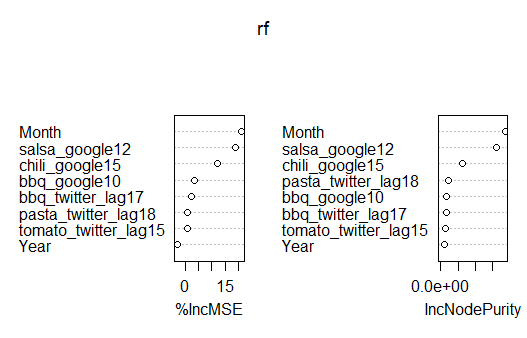
\includegraphics{./figure/RF_V_Imp.png}
\caption{Random Forest Importance}
\end{figure}
The most important features are displayed at the top of this chart, in
this the month was the most important predictor followed closely by
google salsa data at lag 12. This agrees with the importance of monthly
seasonality that we observed in the other models.

\subsection*{Challenger Model -
XGBoost}\label{challenger-model---xgboost}
\addcontentsline{toc}{subsection}{Challenger Model - XGBoost}

XGBoost is an implementation of gradient boosted decision trees designed
for speed and performance. It build trees one at a time, where each new
tree helps to correct errors made by previously trained tree.
\begin{longtable}[]{@{}rrrrr@{}}
\toprule
X & sMAPE & RMSE & X..Bias & Accuracy\tabularnewline
\midrule
\endhead
Train & 15\% & 55311.64 & 11\% & 0.52\tabularnewline
Test & 35\% & 88097.99 & 44\% & 2.00\tabularnewline
\bottomrule
\end{longtable}
\subsection*{Stacking Forecasts}\label{stacking-forecasts}
\addcontentsline{toc}{subsection}{Stacking Forecasts}

Our project focuses only on the ship-to date sales number. The overall
time range from people speaking about keywords on social media, to its
influence on tomato demand, and then to the whole order, manufacture and
ship process takes place for at least 9 months. So we think it's more
meaningful to exclude lags shorter than 9 months. We explored the
correlations between Scholle tomato bag sales and twitter data as well
as Google trend with lags from 9 months up to 24 months, and built
regression with ARIMA model using only the keywords and lags exhibiting
strongly correlations.

Based on discussions with Scholle, we limited the scope to simply the
months of June through October, the months when tomatoes become ripe in
California. We refer to these months as the harvest months.

The stacking method is used to create an additional consensus model by
using the results of trained models. There are two approaches we used
for stacking, simple averaging and creation of a linear model.

We then combined our forecast results from all models mentioned prior in
this report, including the ARIMA model built only on the more stationary
harvest months, the regression with ARIMA errors model using on strong
correlated keywords and lags, random forest model, XGBoost model and
Prophet model. We averaged the forecasts of all combinations of the
models. We found that we were able to improve the model predictions by
combining the Random Forest and Regression with Arima Error models
predictions using a simple average.

The second approach to stacking we attempted was to build a linear model
using the results of all our other models. This model was trained on all
the harvest month data for 2014-2018. The fitted values produced a
better estimate of the actual than the simple average of Random Forest
and Regression with Arima Error. However, we must consider the amount of
information the additional variables add to the regression. When we
applied the step function we achieved a minimized AIC for a linear model
composed of just arima with Regression Error \& Random Forest. The
linear combination of the two slightly weighs more towards the Random
Forest over the Regression with Arima Error.

\chapter*{Conclusion}\label{conclusion}
\addcontentsline{toc}{chapter}{Conclusion}

This section includes a concise summary of the findings. Your summary
might be organized by the research objectives or hypotheses. Make sure
you address the extent to which research objectives are achieved, and if
they are not achieved, explain why. Make sure to interpret your findings
in a way that acknowledges the limitations of the research. That is, do
not extrapolate the insights derived from your research to situations
you have not examined.

\emph{While increasing dosage leads to larger incisor length, the choice
of delivery mechanism between Orange Juice and Vitamin C does not seem
to make a difference. However, at very low levels, Orange Juice appears
more effective, displaying higher average growth.}

\chapter*{Recommendations}\label{recommendations}
\addcontentsline{toc}{chapter}{Recommendations}

Includes guidelines as to ways in which your results should or could be
used in practice. You may discuss other uses of your results, if there
are any. The ways to extend your analysis and the benefits of doing so
might be included in this section as well.

\appendix

\chapter{The First Appendix}\label{the-first-appendix}

This first appendix includes all of the R chunks of code that were
hidden throughout the document (using the \texttt{include\ =\ FALSE}
chunk tag) to help with readibility and/or setup.

\textbf{In section} \ref{pressure-plot}:

\textbf{In section \ref{ref-labels}:}

\chapter{A Second Appendix, for
example}\label{a-second-appendix-for-example}

\chapter*{References}\label{references}
\addcontentsline{toc}{chapter}{References}

Placeholder


% Index?

\end{document}
